% Created 2025-03-30 Sun 13:59
% Intended LaTeX compiler: pdflatex
\documentclass[a4paper, 12pt]{scrartcl}
\usepackage[utf8]{inputenc}
\usepackage[T1]{fontenc}
\usepackage[activate={true,nocompatibility},final,tracking=true,kerning=true,spacing=true,factor=1100,stretch=10,shrink=10]{microtype}
\usepackage[dvipsnames,svgnames]{xcolor}
\usepackage[colorlinks=true, linkcolor=DarkBlue, citecolor=BrickRed, urlcolor=DarkGreen]{hyperref}
\let\oldsection\section
\renewcommand{\section}{\clearpage\oldsection}
\usepackage{graphicx}
\setcounter{secnumdepth}{3}
\author{Rudy Sorensen}
\date{\today}
\title{18-224 Exercise 9}
\hypersetup{
 pdfauthor={Rudy Sorensen},
 pdftitle={18-224 Exercise 9},
 pdfkeywords={},
 pdfsubject={},
 pdfcreator={Emacs 29.4 (Org mode 9.7.11)}, 
 pdflang={English}}

% Setup for code blocks [1/2]

\usepackage{fvextra}

\fvset{%
  commandchars=\\\{\},
  highlightcolor=white!95!black!80!blue,
  breaklines=true,
  breaksymbol=\color{white!60!black}\tiny\ensuremath{\hookrightarrow}}

% Make line numbers smaller and grey.
\renewcommand\theFancyVerbLine{\footnotesize\color{black!40!white}\arabic{FancyVerbLine}}

\usepackage{xcolor}

% In case engrave-faces-latex-gen-preamble has not been run.
\providecolor{EfD}{HTML}{f7f7f7}
\providecolor{EFD}{HTML}{28292e}

% Define a Code environment to prettily wrap the fontified code.
\usepackage[breakable,xparse]{tcolorbox}
\DeclareTColorBox[]{Code}{o}%
{colback=EfD!98!EFD, colframe=EfD!95!EFD,
  fontupper=\footnotesize\setlength{\fboxsep}{0pt},
  colupper=EFD,
  IfNoValueTF={#1}%
  {boxsep=2pt, arc=2.5pt, outer arc=2.5pt,
    boxrule=0.5pt, left=2pt}%
  {boxsep=2.5pt, arc=0pt, outer arc=0pt,
    boxrule=0pt, leftrule=1.5pt, left=0.5pt},
  right=2pt, top=1pt, bottom=0.5pt,
  breakable}

% Support listings with captions
\usepackage{float}
\floatstyle{plain}
\newfloat{listing}{htbp}{lst}
\newcommand{\listingsname}{Listing}
\floatname{listing}{\listingsname}
\newcommand{\listoflistingsname}{List of Listings}
\providecommand{\listoflistings}{\listof{listing}{\listoflistingsname}}


% Setup for code blocks [2/2]: syntax highlighting colors

\newcommand\efstrut{\vrule height 2.1ex depth 0.8ex width 0pt}
\definecolor{EFD}{HTML}{000000}
\definecolor{EfD}{HTML}{ffffff}
\newcommand{\EFD}[1]{\textcolor{EFD}{#1}} % default
\definecolor{EFvp}{HTML}{000000}
\newcommand{\EFvp}[1]{\textcolor{EFvp}{#1}} % variable-pitch
\definecolor{EFh}{HTML}{7f7f7f}
\newcommand{\EFh}[1]{\textcolor{EFh}{#1}} % shadow
\definecolor{EFsc}{HTML}{228b22}
\newcommand{\EFsc}[1]{\textcolor{EFsc}{\textbf{#1}}} % success
\definecolor{EFw}{HTML}{ff8e00}
\newcommand{\EFw}[1]{\textcolor{EFw}{\textbf{#1}}} % warning
\definecolor{EFe}{HTML}{ff0000}
\newcommand{\EFe}[1]{\textcolor{EFe}{\textbf{#1}}} % error
\definecolor{EFl}{HTML}{ff0000}
\newcommand{\EFl}[1]{\textcolor{EFl}{#1}} % link
\definecolor{EFlv}{HTML}{ff0000}
\newcommand{\EFlv}[1]{\textcolor{EFlv}{#1}} % link-visited
\definecolor{EFhi}{HTML}{ff0000}
\newcommand{\EFhi}[1]{\textcolor{EFhi}{#1}} % highlight
\definecolor{EFc}{HTML}{b22222}
\newcommand{\EFc}[1]{\textcolor{EFc}{#1}} % font-lock-comment-face
\definecolor{EFcd}{HTML}{b22222}
\newcommand{\EFcd}[1]{\textcolor{EFcd}{#1}} % font-lock-comment-delimiter-face
\definecolor{EFs}{HTML}{8b2252}
\newcommand{\EFs}[1]{\textcolor{EFs}{#1}} % font-lock-string-face
\definecolor{EFd}{HTML}{8b2252}
\newcommand{\EFd}[1]{\textcolor{EFd}{#1}} % font-lock-doc-face
\definecolor{EFm}{HTML}{008b8b}
\newcommand{\EFm}[1]{\textcolor{EFm}{#1}} % font-lock-doc-markup-face
\definecolor{EFk}{HTML}{9370db}
\newcommand{\EFk}[1]{\textcolor{EFk}{#1}} % font-lock-keyword-face
\definecolor{EFb}{HTML}{483d8b}
\newcommand{\EFb}[1]{\textcolor{EFb}{#1}} % font-lock-builtin-face
\definecolor{EFf}{HTML}{0000ff}
\newcommand{\EFf}[1]{\textcolor{EFf}{#1}} % font-lock-function-name-face
\definecolor{EFv}{HTML}{a0522d}
\newcommand{\EFv}[1]{\textcolor{EFv}{#1}} % font-lock-variable-name-face
\definecolor{EFt}{HTML}{228b22}
\newcommand{\EFt}[1]{\textcolor{EFt}{#1}} % font-lock-type-face
\definecolor{EFo}{HTML}{008b8b}
\newcommand{\EFo}[1]{\textcolor{EFo}{#1}} % font-lock-constant-face
\definecolor{EFwr}{HTML}{ff0000}
\newcommand{\EFwr}[1]{\textcolor{EFwr}{\textbf{#1}}} % font-lock-warning-face
\newcommand{\EFnc}[1]{#1} % font-lock-negation-char-face
\definecolor{EFpp}{HTML}{483d8b}
\newcommand{\EFpp}[1]{\textcolor{EFpp}{#1}} % font-lock-preprocessor-face
\newcommand{\EFrc}[1]{\textbf{#1}} % font-lock-regexp-grouping-construct
\newcommand{\EFrb}[1]{\textbf{#1}} % font-lock-regexp-grouping-backslash
\newcommand{\EFob}[1]{#1} % org-block
\newcommand{\EFobb}[1]{#1} % org-block-begin-line
\newcommand{\EFobe}[1]{#1} % org-block-end-line
\definecolor{EFOa}{HTML}{0000ff}
\newcommand{\EFOa}[1]{\textcolor{EFOa}{#1}} % outline-1
\definecolor{EFOb}{HTML}{a0522d}
\newcommand{\EFOb}[1]{\textcolor{EFOb}{#1}} % outline-2
\definecolor{EFOc}{HTML}{a020f0}
\newcommand{\EFOc}[1]{\textcolor{EFOc}{#1}} % outline-3
\definecolor{EFOd}{HTML}{b22222}
\newcommand{\EFOd}[1]{\textcolor{EFOd}{#1}} % outline-4
\definecolor{EFOe}{HTML}{228b22}
\newcommand{\EFOe}[1]{\textcolor{EFOe}{#1}} % outline-5
\definecolor{EFOf}{HTML}{008b8b}
\newcommand{\EFOf}[1]{\textcolor{EFOf}{#1}} % outline-6
\definecolor{EFOg}{HTML}{483d8b}
\newcommand{\EFOg}[1]{\textcolor{EFOg}{#1}} % outline-7
\definecolor{EFOh}{HTML}{8b2252}
\newcommand{\EFOh}[1]{\textcolor{EFOh}{#1}} % outline-8
\definecolor{EFhn}{HTML}{008b8b}
\newcommand{\EFhn}[1]{\textcolor{EFhn}{#1}} % highlight-numbers-number
\definecolor{EFhq}{HTML}{9370db}
\newcommand{\EFhq}[1]{\textcolor{EFhq}{#1}} % highlight-quoted-quote
\definecolor{EFhs}{HTML}{008b8b}
\newcommand{\EFhs}[1]{\textcolor{EFhs}{#1}} % highlight-quoted-symbol
\definecolor{EFrda}{HTML}{707183}
\newcommand{\EFrda}[1]{\textcolor{EFrda}{#1}} % rainbow-delimiters-depth-1-face
\definecolor{EFrdb}{HTML}{7388d6}
\newcommand{\EFrdb}[1]{\textcolor{EFrdb}{#1}} % rainbow-delimiters-depth-2-face
\definecolor{EFrdc}{HTML}{909183}
\newcommand{\EFrdc}[1]{\textcolor{EFrdc}{#1}} % rainbow-delimiters-depth-3-face
\definecolor{EFrdd}{HTML}{709870}
\newcommand{\EFrdd}[1]{\textcolor{EFrdd}{#1}} % rainbow-delimiters-depth-4-face
\definecolor{EFrde}{HTML}{907373}
\newcommand{\EFrde}[1]{\textcolor{EFrde}{#1}} % rainbow-delimiters-depth-5-face
\definecolor{EFrdf}{HTML}{6276ba}
\newcommand{\EFrdf}[1]{\textcolor{EFrdf}{#1}} % rainbow-delimiters-depth-6-face
\definecolor{EFrdg}{HTML}{858580}
\newcommand{\EFrdg}[1]{\textcolor{EFrdg}{#1}} % rainbow-delimiters-depth-7-face
\definecolor{EFrdh}{HTML}{80a880}
\newcommand{\EFrdh}[1]{\textcolor{EFrdh}{#1}} % rainbow-delimiters-depth-8-face
\definecolor{EFrdi}{HTML}{887070}
\newcommand{\EFrdi}[1]{\textcolor{EFrdi}{#1}} % rainbow-delimiters-depth-9-face
\definecolor{EFdiffa}{HTML}{4F894C}
\newcommand{\EFdiffa}[1]{\textcolor{EFdiffa}{#1}} % diff-added
\definecolor{EFdiffc}{HTML}{842879}
\newcommand{\EFdiffc}[1]{\textcolor{EFdiffc}{#1}} % diff-changed
\definecolor{EFdiffco}{HTML}{525866}
\newcommand{\EFdiffco}[1]{\textcolor{EFdiffco}{#1}} % diff-context
\definecolor{EFdiffr}{HTML}{99324B}
\newcommand{\EFdiffr}[1]{\textcolor{EFdiffr}{#1}} % diff-removed
\definecolor{EFdiffh}{HTML}{398EAC}
\newcommand{\EFdiffh}[1]{\textcolor{EFdiffh}{#1}} % diff-header
\definecolor{EFdifffh}{HTML}{3B6EA8}
\newcommand{\EFdifffh}[1]{\textcolor{EFdifffh}{#1}} % diff-file-header
\definecolor{EFdiffhh}{HTML}{842879}
\newcommand{\EFdiffhh}[1]{\textcolor{EFdiffhh}{#1}} % diff-hunk-header
\begin{document}

\maketitle
\section{Task 1}
\label{sec:org2e91024}
\subsection{Parts E - H}
\label{sec:org932e5b7}
Code is uploaded in repo in file ScanChain\_starter.py
\section{Task 2}
\label{sec:orgf3875b1}
Code for testing adder is in ScanChain\_starter.py. The functions used are adder\_test() and gen\_test\_case(). I did CRT with 20 sets of inputs to verify my work. I don't have any design artifacts besides the output of my tests to prove their correctness. It is after this paragraph. As for reflecting on my work for this task, I don't have much to say. I basically pulled my gen\_test\_case() function from exercise 5 and tweaked it a bit so that the inputs were in the form of a list. This allowed me to easily input my test cases into my input\_chain() function. I then waited a clock cycle and simply had an assertion that compared the value in the x\_out register to the actual sum.

\begin{Code}
\begin{Verbatim}
\color{EFD}TEST \EFhn{0}:
A: [\EFhn{0}, \EFhn{0}, \EFhn{1}, \EFhn{0}]
B: [\EFhn{0}, \EFhn{1}, \EFhn{0}, \EFhn{1}]
X: \EFhn{01110}
CORRECT SUM:0b1110

TEST \EFhn{1}:
A: [\EFhn{1}, \EFhn{1}, \EFhn{0}, \EFhn{0}]
B: [\EFhn{0}, \EFhn{0}, \EFhn{1}, \EFhn{0}]
X: \EFhn{00111}
CORRECT SUM:0b111

TEST \EFhn{2}:
A: [\EFhn{1}, \EFhn{1}, \EFhn{1}, \EFhn{0}]
B: [\EFhn{0}, \EFhn{0}, \EFhn{0}, \EFhn{0}]
X: \EFhn{00111}
CORRECT SUM:0b111

TEST \EFhn{3}:
A: [\EFhn{1}, \EFhn{1}, \EFhn{1}, \EFhn{1}]
B: [\EFhn{1}, \EFhn{0}, \EFhn{0}, \EFhn{1}]
X: \EFhn{11000}
CORRECT SUM:0b11000

TEST \EFhn{4}:
A: [\EFhn{1}, \EFhn{0}, \EFhn{0}, \EFhn{0}]
B: [\EFhn{1}, \EFhn{1}, \EFhn{1}, \EFhn{1}]
X: \EFhn{10000}
CORRECT SUM:0b10000

TEST \EFhn{5}:
A: [\EFhn{0}, \EFhn{0}, \EFhn{1}, \EFhn{0}]
B: [\EFhn{0}, \EFhn{1}, \EFhn{1}, \EFhn{0}]
X: \EFhn{01010}
CORRECT SUM:0b1010

TEST \EFhn{6}:
A: [\EFhn{1}, \EFhn{0}, \EFhn{1}, \EFhn{1}]
B: [\EFhn{0}, \EFhn{1}, \EFhn{0}, \EFhn{1}]
X: \EFhn{10111}
CORRECT SUM:0b10111

TEST \EFhn{7}:
A: [\EFhn{1}, \EFhn{1}, \EFhn{1}, \EFhn{0}]
B: [\EFhn{1}, \EFhn{1}, \EFhn{0}, \EFhn{0}]
X: \EFhn{01010}
CORRECT SUM:0b1010

TEST \EFhn{8}:
A: [\EFhn{0}, \EFhn{0}, \EFhn{0}, \EFhn{1}]
B: [\EFhn{0}, \EFhn{0}, \EFhn{0}, \EFhn{0}]
X: \EFhn{01000}
CORRECT SUM:0b1000

TEST \EFhn{9}:
A: [\EFhn{1}, \EFhn{0}, \EFhn{0}, \EFhn{1}]
B: [\EFhn{1}, \EFhn{0}, \EFhn{0}, \EFhn{0}]
X: \EFhn{01010}
CORRECT SUM:0b1010

TEST \EFhn{10}:
A: [\EFhn{0}, \EFhn{1}, \EFhn{0}, \EFhn{1}]
B: [\EFhn{0}, \EFhn{1}, \EFhn{0}, \EFhn{1}]
X: \EFhn{10100}
CORRECT SUM:0b10100

TEST \EFhn{11}:
A: [\EFhn{1}, \EFhn{1}, \EFhn{0}, \EFhn{0}]
B: [\EFhn{1}, \EFhn{0}, \EFhn{1}, \EFhn{1}]
X: \EFhn{10000}
CORRECT SUM:0b10000

TEST \EFhn{12}:
A: [\EFhn{1}, \EFhn{1}, \EFhn{0}, \EFhn{1}]
B: [\EFhn{0}, \EFhn{0}, \EFhn{0}, \EFhn{0}]
X: \EFhn{01011}
CORRECT SUM:0b1011

TEST \EFhn{13}:
A: [\EFhn{0}, \EFhn{0}, \EFhn{0}, \EFhn{1}]
B: [\EFhn{1}, \EFhn{1}, \EFhn{0}, \EFhn{1}]
X: \EFhn{10011}
CORRECT SUM:0b10011

TEST \EFhn{14}:
A: [\EFhn{0}, \EFhn{0}, \EFhn{0}, \EFhn{0}]
B: [\EFhn{0}, \EFhn{0}, \EFhn{1}, \EFhn{0}]
X: \EFhn{00100}
CORRECT SUM:0b100

TEST \EFhn{15}:
A: [\EFhn{0}, \EFhn{1}, \EFhn{1}, \EFhn{1}]
B: [\EFhn{1}, \EFhn{0}, \EFhn{0}, \EFhn{0}]
X: \EFhn{01111}
CORRECT SUM:0b1111

TEST \EFhn{16}:
A: [\EFhn{0}, \EFhn{0}, \EFhn{1}, \EFhn{0}]
B: [\EFhn{1}, \EFhn{1}, \EFhn{1}, \EFhn{1}]
X: \EFhn{10011}
CORRECT SUM:0b10011

TEST \EFhn{17}:
A: [\EFhn{1}, \EFhn{0}, \EFhn{0}, \EFhn{1}]
B: [\EFhn{0}, \EFhn{0}, \EFhn{1}, \EFhn{0}]
X: \EFhn{01101}
CORRECT SUM:0b1101

TEST \EFhn{18}:
A: [\EFhn{0}, \EFhn{0}, \EFhn{1}, \EFhn{0}]
B: [\EFhn{0}, \EFhn{1}, \EFhn{1}, \EFhn{0}]
X: \EFhn{01010}
CORRECT SUM:0b1010

TEST \EFhn{19}:
A: [\EFhn{0}, \EFhn{0}, \EFhn{0}, \EFhn{0}]
B: [\EFhn{1}, \EFhn{1}, \EFhn{0}, \EFhn{0}]
X: \EFhn{00011}
CORRECT SUM:0b11
\end{Verbatim}
\end{Code}
\section{Task 3}
\label{sec:org1ea27d9}
My code for this task is in ScanChain\_starter.py under the function hidden\_test(). The output of that function is in this document after the reconstructed state diagram. For reflection, I'll start by describing the process. Since I saw that cur\_state was only a 3-bit vector in the .log file and that there was only one 1-bit input, I used the scan chain to feed each possible state in twice, once with data\_avail set to 0 and then again with data\_avail set to 1. Then I simply waited a cycle, used my output\_chain() function to grab the next state out of the cur\_state registers, and printed that alongside the output variables. I think that it was a pretty cool exercise showing how useful scan chains can actually be even with limited knowledge of the design. It was definitely made easier by it being a Moore machine and only having one 1-bit input though.

\begin{center}
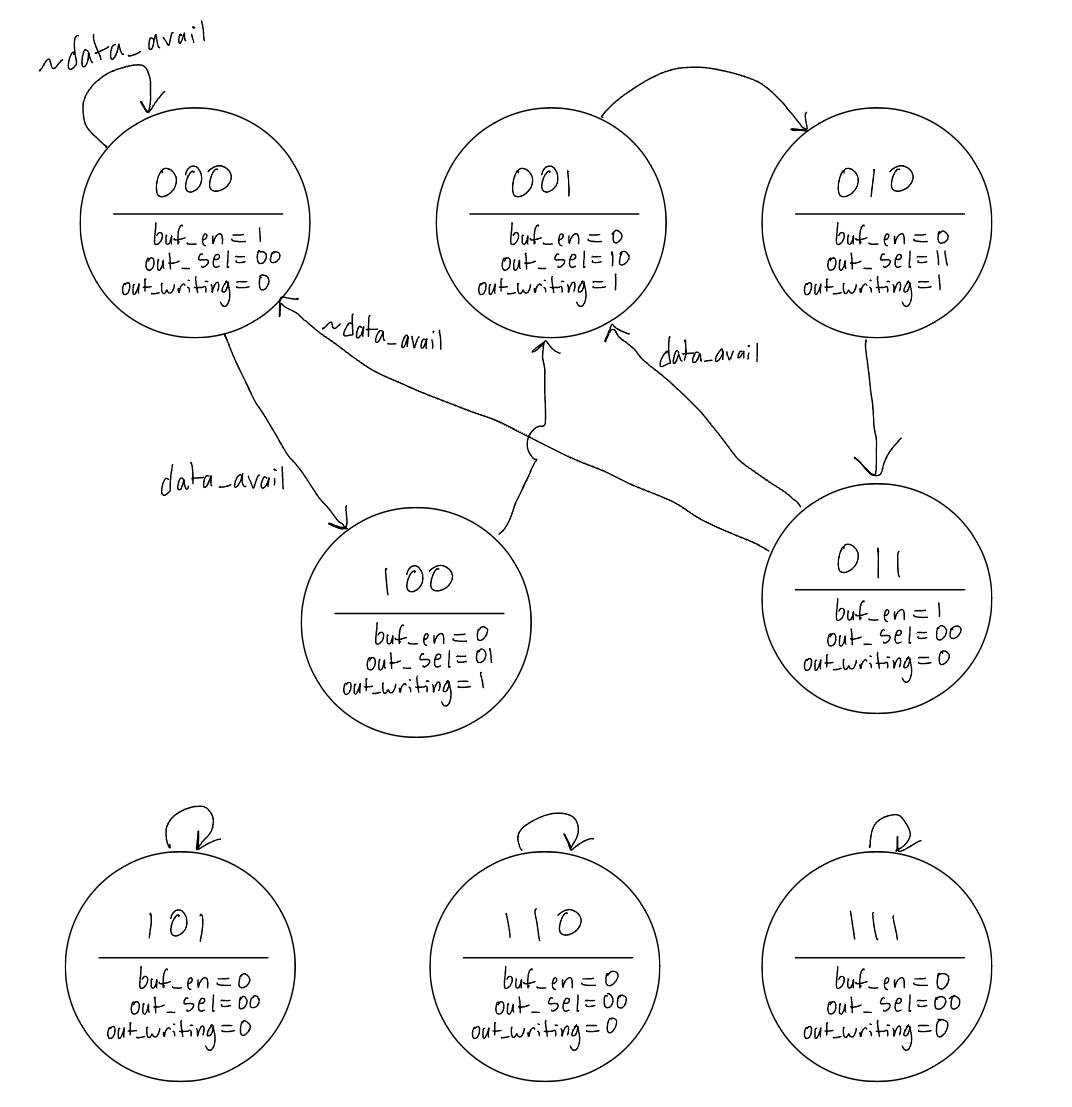
\includegraphics[height=0.75\textwidth]{./ex9_std.jpeg}
\end{center}

\begin{Code}
\begin{Verbatim}
\color{EFD}data\_avail: \EFhn{0}
CURR\_STATE: [\EFhn{0}, \EFhn{0}, \EFhn{0}]
NEXT\_STATE: [\EFhn{0}, \EFhn{0}, \EFhn{0}]
BUF\_EN: \EFhn{1}
OUT\_SEL: \EFhn{00}
OUT\_WRITING: \EFhn{0}

data\_avail: \EFhn{1}
CURR\_STATE: [\EFhn{0}, \EFhn{0}, \EFhn{0}]
NEXT\_STATE: [\EFhn{1}, \EFhn{0}, \EFhn{0}]
BUF\_EN: \EFhn{1}
OUT\_SEL: \EFhn{00}
OUT\_WRITING: \EFhn{0}

data\_avail: \EFhn{0}
CURR\_STATE: [\EFhn{0}, \EFhn{0}, \EFhn{1}]
NEXT\_STATE: [\EFhn{0}, \EFhn{1}, \EFhn{0}]
BUF\_EN: \EFhn{0}
OUT\_SEL: \EFhn{10}
OUT\_WRITING: \EFhn{1}

data\_avail: \EFhn{1}
CURR\_STATE: [\EFhn{0}, \EFhn{0}, \EFhn{1}]
NEXT\_STATE: [\EFhn{0}, \EFhn{1}, \EFhn{0}]
BUF\_EN: \EFhn{0}
OUT\_SEL: \EFhn{10}
OUT\_WRITING: \EFhn{1}

data\_avail: \EFhn{0}
CURR\_STATE: [\EFhn{0}, \EFhn{1}, \EFhn{0}]
NEXT\_STATE: [\EFhn{0}, \EFhn{1}, \EFhn{1}]
BUF\_EN: \EFhn{0}
OUT\_SEL: \EFhn{11}
OUT\_WRITING: \EFhn{1}

data\_avail: \EFhn{1}
CURR\_STATE: [\EFhn{0}, \EFhn{1}, \EFhn{0}]
NEXT\_STATE: [\EFhn{0}, \EFhn{1}, \EFhn{1}]
BUF\_EN: \EFhn{0}
OUT\_SEL: \EFhn{11}
OUT\_WRITING: \EFhn{1}

data\_avail: \EFhn{0}
CURR\_STATE: [\EFhn{0}, \EFhn{1}, \EFhn{1}]
NEXT\_STATE: [\EFhn{0}, \EFhn{0}, \EFhn{0}]
BUF\_EN: \EFhn{1}
OUT\_SEL: \EFhn{00}
OUT\_WRITING: \EFhn{0}

data\_avail: \EFhn{1}
CURR\_STATE: [\EFhn{0}, \EFhn{1}, \EFhn{1}]
NEXT\_STATE: [\EFhn{1}, \EFhn{0}, \EFhn{0}]
BUF\_EN: \EFhn{1}
OUT\_SEL: \EFhn{00}
OUT\_WRITING: \EFhn{0}

data\_avail: \EFhn{0}
CURR\_STATE: [\EFhn{1}, \EFhn{0}, \EFhn{0}]
NEXT\_STATE: [\EFhn{0}, \EFhn{0}, \EFhn{1}]
BUF\_EN: \EFhn{0}
OUT\_SEL: \EFhn{01}
OUT\_WRITING: \EFhn{1}

data\_avail: \EFhn{1}
CURR\_STATE: [\EFhn{1}, \EFhn{0}, \EFhn{0}]
NEXT\_STATE: [\EFhn{0}, \EFhn{0}, \EFhn{1}]
BUF\_EN: \EFhn{0}
OUT\_SEL: \EFhn{01}
OUT\_WRITING: \EFhn{1}

data\_avail: \EFhn{0}
CURR\_STATE: [\EFhn{1}, \EFhn{0}, \EFhn{1}]
NEXT\_STATE: [\EFhn{1}, \EFhn{0}, \EFhn{1}]
BUF\_EN: \EFhn{0}
OUT\_SEL: \EFhn{00}
OUT\_WRITING: \EFhn{0}

data\_avail: \EFhn{1}
CURR\_STATE: [\EFhn{1}, \EFhn{0}, \EFhn{1}]
NEXT\_STATE: [\EFhn{1}, \EFhn{0}, \EFhn{1}]
BUF\_EN: \EFhn{0}
OUT\_SEL: \EFhn{00}
OUT\_WRITING: \EFhn{0}

data\_avail: \EFhn{0}
CURR\_STATE: [\EFhn{1}, \EFhn{1}, \EFhn{0}]
NEXT\_STATE: [\EFhn{1}, \EFhn{1}, \EFhn{0}]
BUF\_EN: \EFhn{0}
OUT\_SEL: \EFhn{00}
OUT\_WRITING: \EFhn{0}

data\_avail: \EFhn{1}
CURR\_STATE: [\EFhn{1}, \EFhn{1}, \EFhn{0}]
NEXT\_STATE: [\EFhn{1}, \EFhn{1}, \EFhn{0}]
BUF\_EN: \EFhn{0}
OUT\_SEL: \EFhn{00}
OUT\_WRITING: \EFhn{0}

data\_avail: \EFhn{0}
CURR\_STATE: [\EFhn{1}, \EFhn{1}, \EFhn{1}]
NEXT\_STATE: [\EFhn{1}, \EFhn{1}, \EFhn{1}]
BUF\_EN: \EFhn{0}
OUT\_SEL: \EFhn{00}
OUT\_WRITING: \EFhn{0}

data\_avail: \EFhn{1}
CURR\_STATE: [\EFhn{1}, \EFhn{1}, \EFhn{1}]
NEXT\_STATE: [\EFhn{1}, \EFhn{1}, \EFhn{1}]
BUF\_EN: \EFhn{0}
OUT\_SEL: \EFhn{00}
OUT\_WRITING: \EFhn{0}
\end{Verbatim}
\end{Code}
\section{Task 4}
\label{sec:org7e15ee6}
\subsection{Part A}
\label{sec:org0751b6d}
Vectors highlighted the same color will catch more than one fault.
\begin{center}
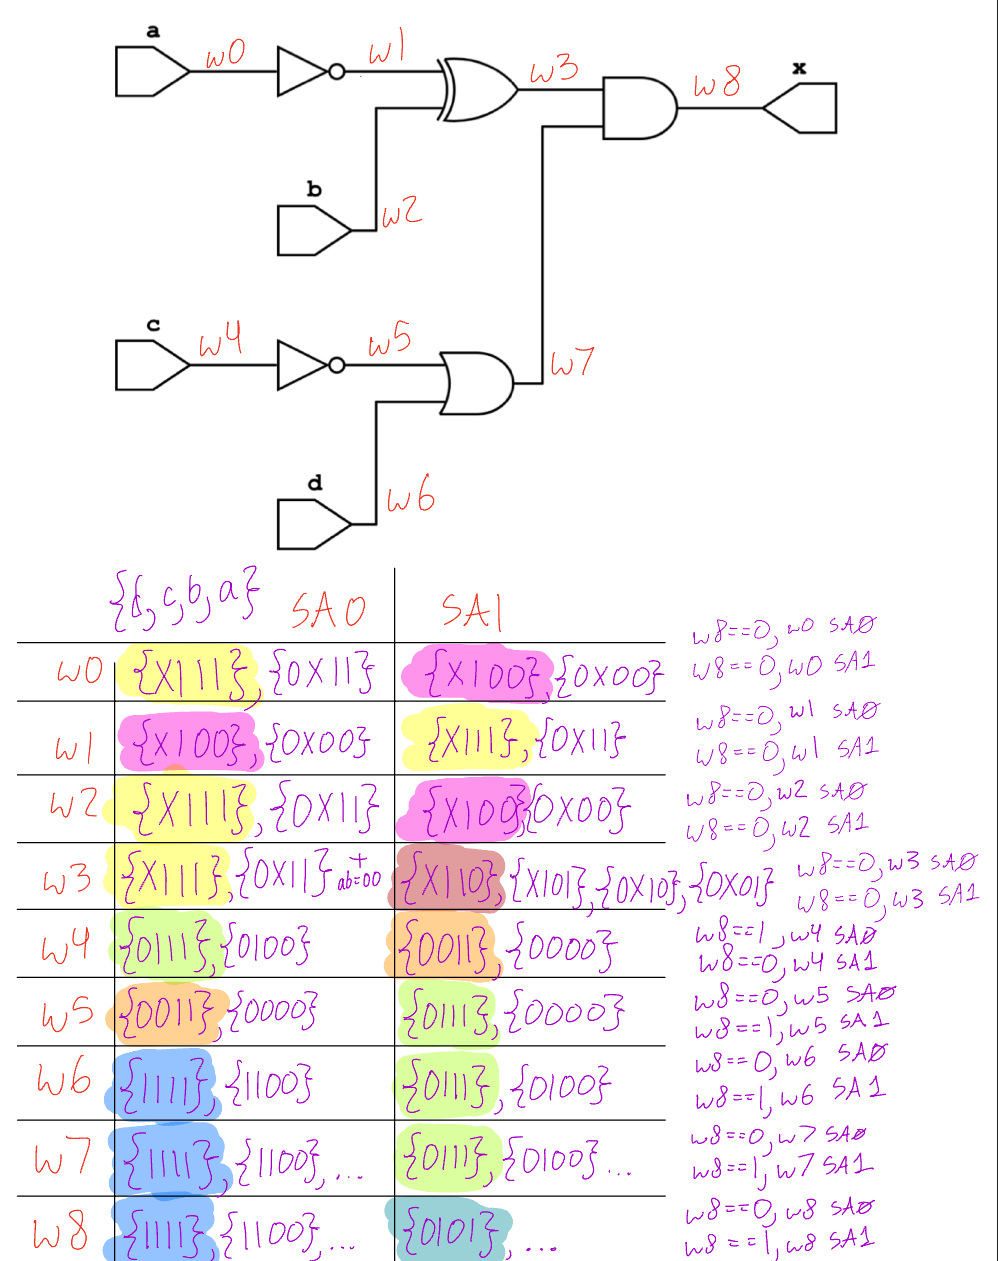
\includegraphics[height=0.95\textwidth]{./ex9_fault_vecs.jpeg}
\end{center}

\newpage
\subsection{Part B}
\label{sec:org496d6db}
\textbf{These outputs are probably wrong. I was confused by this.}\\

For fault1.sv, I had:
\begin{itemize}
\item \textbf{a} possibly SA1
\item \textbf{w1} possibly SA0
\item \textbf{b} possibly SA1\\
\end{itemize}

For fault2.sv I detected no faults.\\

For fault3.sv, I had a variety of possible errors. They were:
\begin{itemize}
\item \textbf{c} possibly SA1
\item \textbf{w5} possibly SA0
\item \textbf{d} possibly SA0
\item \textbf{w7} possibly SA0
\item \textbf{x} possibly SA0\\
\end{itemize}

For fault4.sv, I had that \textbf{x} was SA1.\\

For fault5.sv, I detected no faults.\\
\subsubsection{Outputs}
\label{sec:org9befce5}
\paragraph*{fault1.sv}
\label{sec:org2d71715}
\begin{Code}
\begin{Verbatim}
\color{EFD}VEC: 0b1111
X VAL: \EFhn{1}
A VAL: \EFhn{1}
B VAL: \EFhn{1}
C VAL: \EFhn{1}
D VAL: \EFhn{1}

VEC: 0b1100
X VAL: \EFhn{0}
A VAL: \EFhn{0}
B VAL: \EFhn{0}
C VAL: \EFhn{1}
D VAL: \EFhn{1}
POSSIBLE w0 SA1
POSSIBLE w1 SA0
POSSIBLE w2 SA1

VEC: 0b1110
X VAL: \EFhn{1}
A VAL: \EFhn{0}
B VAL: \EFhn{1}
C VAL: \EFhn{1}
D VAL: \EFhn{1}

VEC: 0b111
X VAL: \EFhn{0}
A VAL: \EFhn{1}
B VAL: \EFhn{1}
C VAL: \EFhn{1}
D VAL: \EFhn{0}

VEC: 0b11
X VAL: \EFhn{1}
A VAL: \EFhn{1}
B VAL: \EFhn{1}
C VAL: \EFhn{0}
D VAL: \EFhn{0}

VEC: 0b1111
X VAL: \EFhn{1}
A VAL: \EFhn{1}
B VAL: \EFhn{1}
C VAL: \EFhn{1}
D VAL: \EFhn{1}

VEC: 0b101
X VAL: \EFhn{0}
A VAL: \EFhn{1}
B VAL: \EFhn{0}
C VAL: \EFhn{1}
D VAL: \EFhn{0}
\end{Verbatim}
\end{Code}

\newpage
\paragraph*{fault2.sv}
\label{sec:org814da1d}
\begin{Code}
\begin{Verbatim}
\color{EFD}VEC: 0b1111
X VAL: \EFhn{1}
A VAL: \EFhn{1}
B VAL: \EFhn{1}
C VAL: \EFhn{1}
D VAL: \EFhn{1}

VEC: 0b1100
X VAL: \EFhn{1}
A VAL: \EFhn{0}
B VAL: \EFhn{0}
C VAL: \EFhn{1}
D VAL: \EFhn{1}

VEC: 0b1110
X VAL: \EFhn{1}
A VAL: \EFhn{0}
B VAL: \EFhn{1}
C VAL: \EFhn{1}
D VAL: \EFhn{1}

VEC: 0b111
X VAL: \EFhn{0}
A VAL: \EFhn{1}
B VAL: \EFhn{1}
C VAL: \EFhn{1}
D VAL: \EFhn{0}

VEC: 0b11
X VAL: \EFhn{1}
A VAL: \EFhn{1}
B VAL: \EFhn{1}
C VAL: \EFhn{0}
D VAL: \EFhn{0}

VEC: 0b1111
X VAL: \EFhn{1}
A VAL: \EFhn{1}
B VAL: \EFhn{1}
C VAL: \EFhn{1}
D VAL: \EFhn{1}

VEC: 0b101
X VAL: \EFhn{0}
A VAL: \EFhn{1}
B VAL: \EFhn{0}
C VAL: \EFhn{1}
D VAL: \EFhn{0}
\end{Verbatim}
\end{Code}

\newpage
\paragraph*{fault3.sv}
\label{sec:org5006ba0}
\begin{Code}
\begin{Verbatim}
\color{EFD}VEC: 0b1111
X VAL: \EFhn{0}
A VAL: \EFhn{1}
B VAL: \EFhn{1}
C VAL: \EFhn{1}
D VAL: \EFhn{1}
POSSIBLE w0 SA0
POSSIBLE w1 SA1
POSSIBLE w2 SA0
POSSIBLE w3 SA0

VEC: 0b1100
X VAL: \EFhn{0}
A VAL: \EFhn{0}
B VAL: \EFhn{0}
C VAL: \EFhn{1}
D VAL: \EFhn{1}
POSSIBLE w0 SA1
POSSIBLE w1 SA0
POSSIBLE w2 SA1

VEC: 0b1110
X VAL: \EFhn{0}
A VAL: \EFhn{0}
B VAL: \EFhn{1}
C VAL: \EFhn{1}
D VAL: \EFhn{1}
POSSIBLE w3 SA1

VEC: 0b111
X VAL: \EFhn{0}
A VAL: \EFhn{1}
B VAL: \EFhn{1}
C VAL: \EFhn{1}
D VAL: \EFhn{0}

VEC: 0b11
X VAL: \EFhn{0}
A VAL: \EFhn{1}
B VAL: \EFhn{1}
C VAL: \EFhn{0}
D VAL: \EFhn{0}
POSSIBLE w4 SA1
POSSIBLE w5 SA0

VEC: 0b1111
X VAL: \EFhn{0}
A VAL: \EFhn{1}
B VAL: \EFhn{1}
C VAL: \EFhn{1}
D VAL: \EFhn{1}
POSSIBLE w6 SA0
POSSIBLE w7 SA0
POSSIBLE w8 SA0

VEC: 0b101
X VAL: \EFhn{0}
A VAL: \EFhn{1}
B VAL: \EFhn{0}
C VAL: \EFhn{1}
D VAL: \EFhn{0}
\end{Verbatim}
\end{Code}

\newpage
\paragraph*{fault4.sv}
\label{sec:org80a1927}
\begin{Code}
\begin{Verbatim}
\color{EFD}VEC: 0b1111
X VAL: \EFhn{1}
A VAL: \EFhn{1}
B VAL: \EFhn{1}
C VAL: \EFhn{1}
D VAL: \EFhn{1}

VEC: 0b1100
X VAL: \EFhn{1}
A VAL: \EFhn{0}
B VAL: \EFhn{0}
C VAL: \EFhn{1}
D VAL: \EFhn{1}

VEC: 0b1110
X VAL: \EFhn{1}
A VAL: \EFhn{0}
B VAL: \EFhn{1}
C VAL: \EFhn{1}
D VAL: \EFhn{1}

VEC: 0b111
X VAL: \EFhn{1}
A VAL: \EFhn{1}
B VAL: \EFhn{1}
C VAL: \EFhn{1}
D VAL: \EFhn{0}
POSSIBLE w4 SA0
POSSIBLE w5 SA1
POSSIBLE w6 SA1
POSSIBLE w7 SA1

VEC: 0b11
X VAL: \EFhn{1}
A VAL: \EFhn{1}
B VAL: \EFhn{1}
C VAL: \EFhn{0}
D VAL: \EFhn{0}

VEC: 0b1111
X VAL: \EFhn{1}
A VAL: \EFhn{1}
B VAL: \EFhn{1}
C VAL: \EFhn{1}
D VAL: \EFhn{1}

VEC: 0b101
X VAL: \EFhn{1}
A VAL: \EFhn{1}
B VAL: \EFhn{0}
C VAL: \EFhn{1}
D VAL: \EFhn{0}
POSSIBLE w8 SA1
\end{Verbatim}
\end{Code}

\newpage
\paragraph*{fault5.sv}
\label{sec:org58a3cd9}
\begin{Code}
\begin{Verbatim}
\color{EFD}VEC: 0b1111
X VAL: \EFhn{1}
A VAL: \EFhn{1}
B VAL: \EFhn{1}
C VAL: \EFhn{1}
D VAL: \EFhn{1}

VEC: 0b1100
X VAL: \EFhn{1}
A VAL: \EFhn{0}
B VAL: \EFhn{0}
C VAL: \EFhn{1}
D VAL: \EFhn{1}

VEC: 0b1110
X VAL: \EFhn{0}
A VAL: \EFhn{0}
B VAL: \EFhn{1}
C VAL: \EFhn{1}
D VAL: \EFhn{1}
POSSIBLE w3 SA1

VEC: 0b111
X VAL: \EFhn{0}
A VAL: \EFhn{1}
B VAL: \EFhn{1}
C VAL: \EFhn{1}
D VAL: \EFhn{0}

VEC: 0b11
X VAL: \EFhn{1}
A VAL: \EFhn{1}
B VAL: \EFhn{1}
C VAL: \EFhn{0}
D VAL: \EFhn{0}

VEC: 0b1111
X VAL: \EFhn{1}
A VAL: \EFhn{1}
B VAL: \EFhn{1}
C VAL: \EFhn{1}
D VAL: \EFhn{1}

VEC: 0b101
X VAL: \EFhn{0}
A VAL: \EFhn{1}
B VAL: \EFhn{0}
C VAL: \EFhn{1}
D VAL: \EFhn{0}
\end{Verbatim}
\end{Code}
\end{document}
